%\documentclass[12pt]{beamer}
\documentclass[handout, 12pt]{beamer}

% theme
\usetheme{default}

% packages
\usepackage{tikz}
\usepackage{graphicx}
\usepackage{hyperref}
\usepackage{amsmath, amsfonts}

% macros
\newcommand{\N}{\mathbb{N}}
\newcommand{\R}{\mathbb{R}}
\newcommand{\br}[1]{\mathopen{}\left(#1\right)\mathclose{}}
\newcommand{\bigo}[1]{\mathcal{O}\br{#1}}

% colors
\definecolor{r}{rgb}{0.87, 0.2, 0.2}

% metadata
\title{The Limits of Computation}
\subtitle{or\\``a fascinating tale of infinity and paradox''}
\author{George Papamakarios}
\date{}

\begin{document}

\frame{\titlepage}

%%%%%%%%%%%%%%%%%%%%%%%%%%%%%%%%%%%%%%%%%%%%%%%%%%%%%%%%%%%%%%%%%%%%%%%%%%%%%%%%%%%%
\begin{frame}

\frametitle{A fundamental question\ldots}

\centering
{\Large What can computers do?}

\end{frame}

%%%%%%%%%%%%%%%%%%%%%%%%%%%%%%%%%%%%%%%%%%%%%%%%%%%%%%%%%%%%%%%%%%%%%%%%%%%%%%%%%%%%
\begin{frame}<beamer:0>

\footnotesize
We created computers to help us solve \textbf{problems}, and computers have done that astonishingly well. But since the early days of computation, i.e.~the first half of the 20th century, people wondered whether there are any problems that computers couldn't solve.
\\[0.6em]
This is a fundamental question in theoretical computer science; can computers solve any computational problem? Or are there problems that no algorithm can ever solve? Similarly to asking what shapes we can construct with a ruler and a compass, we ask what problems we can solve with devices capable of computation. Can we solve them all? Or, like with ruler-and-compass constructions, there is a limit?
\\[0.6em]
We will start by spilling the beans and answering this question straight away\ldots

\end{frame}

%%%%%%%%%%%%%%%%%%%%%%%%%%%%%%%%%%%%%%%%%%%%%%%%%%%%%%%%%%%%%%%%%%%%%%%%%%%%%%%%%%%%
\begin{frame}

\frametitle{\ldots and the answer!}

\begin{block}{}
\centering
\color{r}{\LARGE There exist problems that no algorithm can solve!}
\end{block}

\pause

\begin{block}{}
\centering
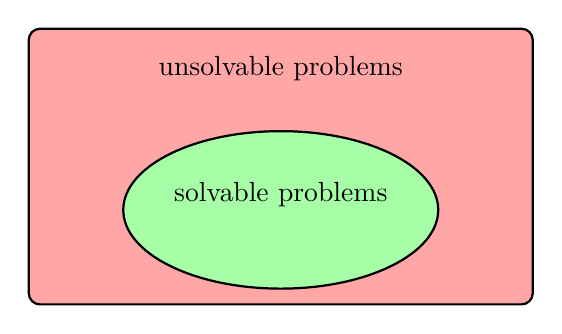
\begin{tikzpicture}

\draw[rounded corners=4pt,thick,fill=red!35!white] (-3.2,0) rectangle (3.2,3.5);
\node at (0,3) {unsolvable problems};

\draw[thick,fill=green!35!white] (0,1.2) ellipse (2 and 1);
\node at (0,1.4) {solvable problems};

\end{tikzpicture}
\end{block}

\end{frame}

%%%%%%%%%%%%%%%%%%%%%%%%%%%%%%%%%%%%%%%%%%%%%%%%%%%%%%%%%%%%%%%%%%%%%%%%%%%%%%%%%%%%
\begin{frame}<beamer:0>

\footnotesize
The answer to whether computation is all-powerful is a big, cold-hearted \textbf{no}. There are problems, and by that I mean \textbf{computational} problems, that no algorithm can possibly solve.
\\[0.6em]
Several questions naturally arise. Why is this the case? What do these unsolvable problems look like? Should we care about them? Where does the boundary between solvable and unsolvable problems lie?

\end{frame}

%%%%%%%%%%%%%%%%%%%%%%%%%%%%%%%%%%%%%%%%%%%%%%%%%%%%%%%%%%%%%%%%%%%%%%%%%%%%%%%%%%%%
\begin{frame}

\frametitle{Two proofs}

\begin{itemize}
\addtolength{\itemsep}{1\baselineskip}
\item Proof \#1: The \textbf{infinity} proof
\item Proof \#2: The \textbf{paradox} proof
\end{itemize}

\end{frame}

%%%%%%%%%%%%%%%%%%%%%%%%%%%%%%%%%%%%%%%%%%%%%%%%%%%%%%%%%%%%%%%%%%%%%%%%%%%%%%%%%%%%
\begin{frame}<beamer:0>

\footnotesize
We're going to discuss two proofs (or rather proof sketches) of the statement that unsolvable problems exist. These will provide some insight into the questions we asked above.
\\[0.6em]
The first proof, I call it ``the infinity proof'', is \textbf{non-constructive}; it will prove the existence of unsolvable problems without naming any of them! The idea behind the proof is embarassingly simple: we will just \textbf{count} all possible programs and all possible problems. We will discover that there are more problems than programs, and hence conclude that there simply aren't enough programs to solve them all!
\\[0.6em]
The second proof, I call it ``the paradox proof'', is \textbf{constructive}. We will consider a specific problem, the notorious \textbf{halting problem}, and we will show that if a program can solve it, then logical mayhem will follow! Hence, the halting problem will be shown to be unsolvable by contradiction.

\end{frame}

%%%%%%%%%%%%%%%%%%%%%%%%%%%%%%%%%%%%%%%%%%%%%%%%%%%%%%%%%%%%%%%%%%%%%%%%%%%%%%%%%%%%
\begin{frame}

\frametitle{The infinity proof}

\begin{block}{Step 1: count all programs}

\begin{itemize}
\addtolength{\itemsep}{0.2\baselineskip}
\pause\item A program is a string.
\pause\item There are infinitely many strings\ldots
\pause\item \ldots but countably many; strings are \textbf{listable}.
\pause\item \color{r}{There are as many programs as numbers in $\N$.}
\end{itemize}
\end{block}

\end{frame}

%%%%%%%%%%%%%%%%%%%%%%%%%%%%%%%%%%%%%%%%%%%%%%%%%%%%%%%%%%%%%%%%%%%%%%%%%%%%%%%%%%%%
\begin{frame}

\frametitle{The infinity proof}

\begin{block}{Step 2: count all problems}

\begin{itemize}
\addtolength{\itemsep}{0.2\baselineskip}
\pause\item A problem is a (desired) transformation from an input to an output.
\pause\item Inputs and outputs are strings.
\pause\item Strings are isomorphic to $\N$\ldots
\pause\item \ldots hence problems are mappings from $\N$ to $\N$\ldots
\pause\item \ldots which in turn are isomorphic to $\R$.
\pause\item \color{r}{There are as many problems as numbers in $\R$.}
\end{itemize}

\end{block}

\end{frame}

%%%%%%%%%%%%%%%%%%%%%%%%%%%%%%%%%%%%%%%%%%%%%%%%%%%%%%%%%%%%%%%%%%%%%%%%%%%%%%%%%%%%
\begin{frame}

\frametitle{The infinity proof}

\begin{block}{\ldots and the punchline}
\centering
\vspace{1.5em}
{\large elements in $\R$ $>$ elements in $\N$}
\end{block}

\begin{block}{}
\centering
\color{r}{\large QED}
\end{block}

\end{frame}

%%%%%%%%%%%%%%%%%%%%%%%%%%%%%%%%%%%%%%%%%%%%%%%%%%%%%%%%%%%%%%%%%%%%%%%%%%%%%%%%%%%%
\begin{frame}

\frametitle{A shocking realization}

\begin{block}{}
\centering
\color{r}{\LARGE Almost all problems are unsolvable!}
\end{block}

\pause

\begin{block}{}
\centering
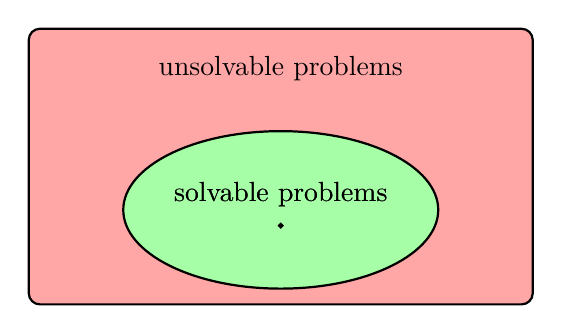
\begin{tikzpicture}

\draw[rounded corners=4pt,thick,fill=red!35!white] (-3.2,0) rectangle (3.2,3.5);
\node at (0,3) {unsolvable problems};

\draw<2>[thick,fill=green!35!white] (0,1.2) ellipse (2 and 1);
\node<2> at (0,1.4) {solvable problems};

\draw<3>[thick,fill=green!35!white] (0,1) ellipse (0.02 and 0.02);
\node<3> at (0,1.4) {solvable problems};

\end{tikzpicture}
\end{block}

\end{frame}

%%%%%%%%%%%%%%%%%%%%%%%%%%%%%%%%%%%%%%%%%%%%%%%%%%%%%%%%%%%%%%%%%%%%%%%%%%%%%%%%%%%%
\begin{frame}<beamer:0>

\footnotesize
We've shown, simply by counting, that the set of programs is isomorphic to $\N$ and the set of problems is isomorphic to $\R$. We know that there are more elements in $\R$ than in $\N$, in the sense that $\N\subset\R$ and there is no injective mapping from $\N$ to $\R$. Hence there simply aren't enough programs to solve all problems; \textbf{unsolvable problems must exist!}
\\[0.6em]
But the result is even more shocking than that. We know that, in a measure-theoretic sense, almost all real numbers are not integers. In other words, the probability that a randomly chosen real number is an integer is $0$. Hence, the chances that a randomly chosen problem is solvable are negligible; \textbf{almost all problems are unsolvable!}

\end{frame}

%%%%%%%%%%%%%%%%%%%%%%%%%%%%%%%%%%%%%%%%%%%%%%%%%%%%%%%%%%%%%%%%%%%%%%%%%%%%%%%%%%%%
\begin{frame}

\frametitle{Wait a minute\ldots}

\begin{itemize}
\addtolength{\itemsep}{0.5\baselineskip}
\pause\item So are computers totally useless?
\pause\item Real-life problems have \textbf{structure}.
\pause\item We can only \textbf{describe} countably many problems!
\end{itemize}

\end{frame}

%%%%%%%%%%%%%%%%%%%%%%%%%%%%%%%%%%%%%%%%%%%%%%%%%%%%%%%%%%%%%%%%%%%%%%%%%%%%%%%%%%%%
\begin{frame}<beamer:0>

\footnotesize
So are computers totally useless? That seems to be the conclusion of our reasoning, since we've said that computers can solve almost no problems. Yet our experience with them says otherwise; what is going on here?
\\[0.6em]
The reason for this result is that we counted as problems \textbf{arbitrary mappings} from $\N$ to $\N$. Real problems we care about are not arbitrary mappings, they have some \textbf{structure}. After all, we can only describe countably many problems! It's easy to see why; just observe that the description of a problem, be it in English or in a formal language, is a string, and there are countably many of them. Hence the problems that we can actually talk about, and possibly care about, are as many as numbers in $\N$, as many as programs! Perhaps then we can solve them all!
\\[0.6em]
This is indeed reassuring, but we will still see that it is not the case. There are problems that we can easily describe and are of practical interest that are still unsolvable. The infamous \textbf{halting problem} is one of them.

\end{frame}

%%%%%%%%%%%%%%%%%%%%%%%%%%%%%%%%%%%%%%%%%%%%%%%%%%%%%%%%%%%%%%%%%%%%%%%%%%%%%%%%%%%%
\begin{frame}[fragile]

\frametitle{The paradox proof}

\begin{block}{The halting problem}
Given a program \texttt{P} and an input \texttt{x}, does \texttt{P} halt when run with input \texttt{x}?
\end{block}

\pause

\begin{block}{}
\begin{columns}[c] 
\begin{column}{0.4\textwidth}
A program that halts
\begin{verbatim}
1.  P(x):
2.     print x
3.  end  
  
\end{verbatim}
\end{column}
\hspace{-2.3em}\vrule\hspace{2.3em}
\begin{column}{0.4\textwidth}
A program that doesn't
\begin{verbatim}
1.  P(x):
2.     while True:
3.        print x
4.  end
\end{verbatim}
\end{column}
\end{columns}
\end{block}

\end{frame}

%%%%%%%%%%%%%%%%%%%%%%%%%%%%%%%%%%%%%%%%%%%%%%%%%%%%%%%%%%%%%%%%%%%%%%%%%%%%%%%%%%%%
\begin{frame}

\frametitle{The paradox proof}

\begin{block}{Step 1: postulate}
\pause
Suppose that \texttt{halt(P,x)} solves the halting problem.
\begin{equation*}
\texttt{halt(P,x)} = \begin{cases}
\texttt{yes} & \text{if \texttt{P(x)} halts} \\
\texttt{no} & \text{if \texttt{P(x)} loops} \\
\end{cases}
\end{equation*}
\end{block}

\end{frame}

%%%%%%%%%%%%%%%%%%%%%%%%%%%%%%%%%%%%%%%%%%%%%%%%%%%%%%%%%%%%%%%%%%%%%%%%%%%%%%%%%%%%
\begin{frame}[fragile]

\frametitle{The paradox proof}
\begin{block}{Step 2: construct the program of doom}
\pause
\begin{verbatim}
     1.  doom(P):
     2.    if halt(P,P) == yes:
     3.        loop forever
     4.     else:
     5.        return
     6.  end
\end{verbatim}
\end{block}

\end{frame}

%%%%%%%%%%%%%%%%%%%%%%%%%%%%%%%%%%%%%%%%%%%%%%%%%%%%%%%%%%%%%%%%%%%%%%%%%%%%%%%%%%%%
\begin{frame}[fragile]

\frametitle{The paradox proof}

\begin{block}{Step 3: pull the trigger}
\pause
What happens if we run \texttt{doom(doom)}?
\pause
\begin{verbatim}
     1.  doom(doom):
     2.    if halt(doom,doom) == yes:
     3.        loop forever
     4.     else:
     5.        return
     6.  end
\end{verbatim}
\pause
\texttt{doom(doom)} halts when it loops, and it loops when it halts!
\end{block}

\end{frame}

%%%%%%%%%%%%%%%%%%%%%%%%%%%%%%%%%%%%%%%%%%%%%%%%%%%%%%%%%%%%%%%%%%%%%%%%%%%%%%%%%%%%
\begin{frame}

\frametitle{The paradox proof}

\begin{block}{\ldots and the punchline}
\centering
\vspace{1.5em}
{\large By contradiction \texttt{halt(P,x)} cannot exist!}
\end{block}

\begin{block}{}
\centering
\color{r}{\large QED}
\end{block}

\pause

\begin{block}{}
\begin{columns}[c] 
\begin{column}{0.5\textwidth}
\raggedleft
Alan Turing\\
1936
\end{column}
\begin{column}{0.6\textwidth}
\raggedright
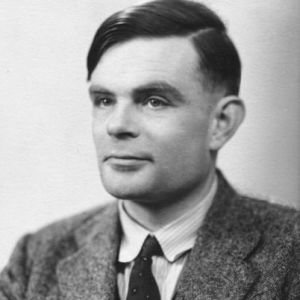
\includegraphics[width=7em]{pics/alan_turing.jpg}
\end{column}
\end{columns}
\end{block}

\end{frame}

%%%%%%%%%%%%%%%%%%%%%%%%%%%%%%%%%%%%%%%%%%%%%%%%%%%%%%%%%%%%%%%%%%%%%%%%%%%%%%%%%%%%
\begin{frame}<beamer:0>

\footnotesize
We've proved that the halting problem is unsolvable by \textbf{contradiction}. That is, we showed that the existence of a program that solves it leads to paradoxical results. This is a sketch of a famous proof by \textbf{Alan Turing} published in \textbf{1936}. Turing introduced the \textbf{Turing machine}, a theoretical computing device which formalizes the notion of a program (in our proof sketch we used the notion of a program informally). Then, he went on to show that no Turing machine can determine whether a given Turing machine halts on a given input. It is remarkable that this proof dates back to 1936; computers barely existed back then!
\\[0.6em]
It is worth mentioning that the reason Turing was interested in computability is David Hilbert's \textbf{Entscheidungsproblem}, which asks for an algorithm to determine whether a statement of first order logic can be derived from a set of axioms. The undecidability of the halting problem implies the undecidability of the Entscheidungsproblem, which is exctly what Turing set out to prove. At the same time as Turing, in 1936, Alonzo Church (Turing's PhD supervisor!) published an equivalent proof of the undecidability of the Entscheidungsproblem using lambda calculus.

\end{frame}

%%%%%%%%%%%%%%%%%%%%%%%%%%%%%%%%%%%%%%%%%%%%%%%%%%%%%%%%%%%%%%%%%%%%%%%%%%%%%%%%%%%%
\begin{frame}

\frametitle{Other unsolvable problems}

\begin{itemize}
\addtolength{\itemsep}{1\baselineskip}
\pause\item \textbf{The verification problem}: Given a program and a specification, does the program follow the specification?
\pause\item \textbf{The Entscheidungsproblem}: Given a set of axioms and a statement of first order logic, does the statement follow from the axioms?
\pause\item \textbf{The number theory problem}: Given a statement of number theory, is it true?
\end{itemize}

\end{frame}

%%%%%%%%%%%%%%%%%%%%%%%%%%%%%%%%%%%%%%%%%%%%%%%%%%%%%%%%%%%%%%%%%%%%%%%%%%%%%%%%%%%%
\begin{frame}<beamer:0>

\footnotesize
Having shown one particular problem to be unsolvable, we can use \textbf{reduction} to show other problems to be unsolvable too.
\\[0.6em]
The \textbf{verification problem} asks whether a given program follows a given specification. This would be a great way to check the correctness of our programs! However, we can show that if there is a program that solves it, then the halting problem becomes solvable too. Suppose you want to know if program \texttt{P} halts with input \texttt{x}. Then construct a program \texttt{Q} which first simulates \texttt{P(x)} and then returns $0$. Notice that \texttt{Q} will return $0$ if and only if \texttt{P(x)} halts. If you can solve the verification problem, then you can ask ``does \texttt{Q} return $0$'' and immediately solve the halting problem, which is a contradiction.
\\[0.6em]
The \textbf{Entscheidungsproblem} was posed by \textbf{David Hilbert} in \textbf{1928}, hoping (as it turned out, in vain) for a positive answer to it. We can show that a program which solves the Entscheidungsproblem leads to a program which solves the halting problem. If you want to determine whether \texttt{P(x)} halts, construct a statement in first-order logic with the meaning ``there exists a number of steps after which \texttt{P(x)} halts'' and use your solution to the Entscheidungsproblem to answer this, which leads to a contradiction.

\end{frame}

%%%%%%%%%%%%%%%%%%%%%%%%%%%%%%%%%%%%%%%%%%%%%%%%%%%%%%%%%%%%%%%%%%%%%%%%%%%%%%%%%%%%
\begin{frame}<beamer:0>

\footnotesize
Finally, a solution to the \textbf{number theory problem} would provide an automatic way to prove or disprove any statement of number theory! If a program solved it, then we would simply feed into it Fermat's last theorem, Goldbach's conjecture, the abc conjecture, or any other proposition of number theory we wanted to know whether it's true, wait for some time (maybe long, but still finitely long!) and get a definite answer. However, no such program exists, and this is a direct consequence of \textbf{G\"{o}del's first incompleteness theorem} (published in 1931), which says that no automatic procedure can generate all true statements of number theory and only them. If such a program existed that would immediately provide such an automatic procedure, which would be a contradiction.

\end{frame}

%%%%%%%%%%%%%%%%%%%%%%%%%%%%%%%%%%%%%%%%%%%%%%%%%%%%%%%%%%%%%%%%%%%%%%%%%%%%%%%%%%%%
\begin{frame}<beamer:0>

\footnotesize
The above problems give us a flavour of the type of problems that computers cannot solve. They typically contain some element of \textbf{infinity} in their computational requirements. For instance, one way to ``solve'' the halting problem would be to run \texttt{P(x)} for long enough and see whether it halts. This might require running it forever, in case it doesn't halt! Similarly, ``solving'' the verification problem might require running a program for infinitely long or for infinitely many inputs to see if the specification is met. A program ``solving'' the Entscheidungsproblem could generate all statements that follow from the axioms and check whether the given statement is included in them. Since infinitely many statements can be generated from the axioms, this procedure might take infinitely long. Finally, in ``proving'' a number-theoretic proposition such as ``there exist infinitely many primes'', a program would have to go through all numbers in $\N$ which of course would take infinitely long.
\\[0.6em]
Ultimately, the limits of computation are due to the fact that \textbf{we require programs to run in finite time}. If we allowed programs to run infinitely long, such problems would become solvable. But clearly, a program running infinitely long is a rather useless one.

\end{frame}

%%%%%%%%%%%%%%%%%%%%%%%%%%%%%%%%%%%%%%%%%%%%%%%%%%%%%%%%%%%%%%%%%%%%%%%%%%%%%%%%%%%%
\begin{frame}

\frametitle{Takeaways}

\begin{itemize}
\addtolength{\itemsep}{1\baselineskip}
\pause\item Is computation limited? {\color{r} Yes}
\pause\item Do unsolvable problems include problems we care about? {\color{r} Yes}
\pause\item Am I going to stumble across any unsolvable problems in my work? {\color{r} Probably not!}
\end{itemize}

\end{frame}

\end{document}
